\nonumchapter{学生实验}

\nonumsection{化学实验的目的}\label{sec:xssy-mudi}

化学是一门以实验为基础的科学。化学实验在化学教学中占有十分重要的地位。
通过化学实验可以帮助学生形成化学概念,理解和巩固化学知识,
正确地掌握实验的基本方法和基本技能,对培养学生的观察、思维、独立操作等能力,
理论联系实际的学风和实事求是、严肃认真的科学态度以及探讨问题的科学方法都有重要的意义。
化学实验是化学教学不可分割的一个重要组成部分,不做实验或少做实验,实际教学效果是不会好的。


\nonumsection{学生实验的要求}\label{sec:xssy-yaoqiu}

学生必须亲自动手做实验。为了保证学生实验课能够顺利地进行, 提高实验教学质量, 实验时必须注意下面几个问题:

1. 上实验课前,要复习课文里的有关内容,阅读实验说明,理解实验目的,明了实验步骤和注意事项。

对于实验习题,要预先经过研究,然后提出解决的方案和需用的仪器和药品。

2. 做实验以前,要检查实验用品是不是齐全。桌上的实验用品要摆得整齐。

3. 做实验的时候,必须按照实验说明的步骤和方法进行,必须遵从教师的指导。

4. 要注意安全。要遵守实验操作规程,特别是实验说明里有关预防发生事故的规定。要谨慎、妥善地处理腐蚀性物质和易燃、易爆、有毒的物质。

5. 要保持实验室里的安静,自觉地遵守纪律。要爱护公共财物和仪器设备。要注意节约药品。

6. 做实验的时候,要认真地和耐心细致地观察与实验目的要求有关的现象,分析现象发生的原因。
对于实验的内容、观察到的现象和得出的结论,都要实事求是地随时作记录。

7. 做完实验后,要认真地写出实验报告。实验报告可以参照下面的格式:

\begin{table}[H]
    \centering
    {\Large 化学实验报告}

    班级 \xhx[5em] 姓名 \xhx[5em] 日期  \xhx[5em] \\[1em]

    \begin{minipage}{12cm}
        实验名称:

        实验目的:

        \vspace*{1em}\begin{tblr}{
            vlines,
            hline{1}={1.5pt,solid},
            hline{2}={solid},
            vline{1,4}={1.5pt,solid},
        }
            实验的内容和装置图 & 观察到的现象 & 结论、解释和化学方程式 \\
            & &
        \end{tblr}

    \end{minipage}

\end{table}

8. 做完实验,拆开实验装置,把仪器里没有用的物质倒在废液缸里,把有用的物质倒在指定的容器里。
然后把仪器洗涤干净放回原处,把实验桌收拾干净。


\nonumsection{化学实验的常用仪器}\label{sec:xssy-yiqi}

\begin{figure}[H]
    \centering
    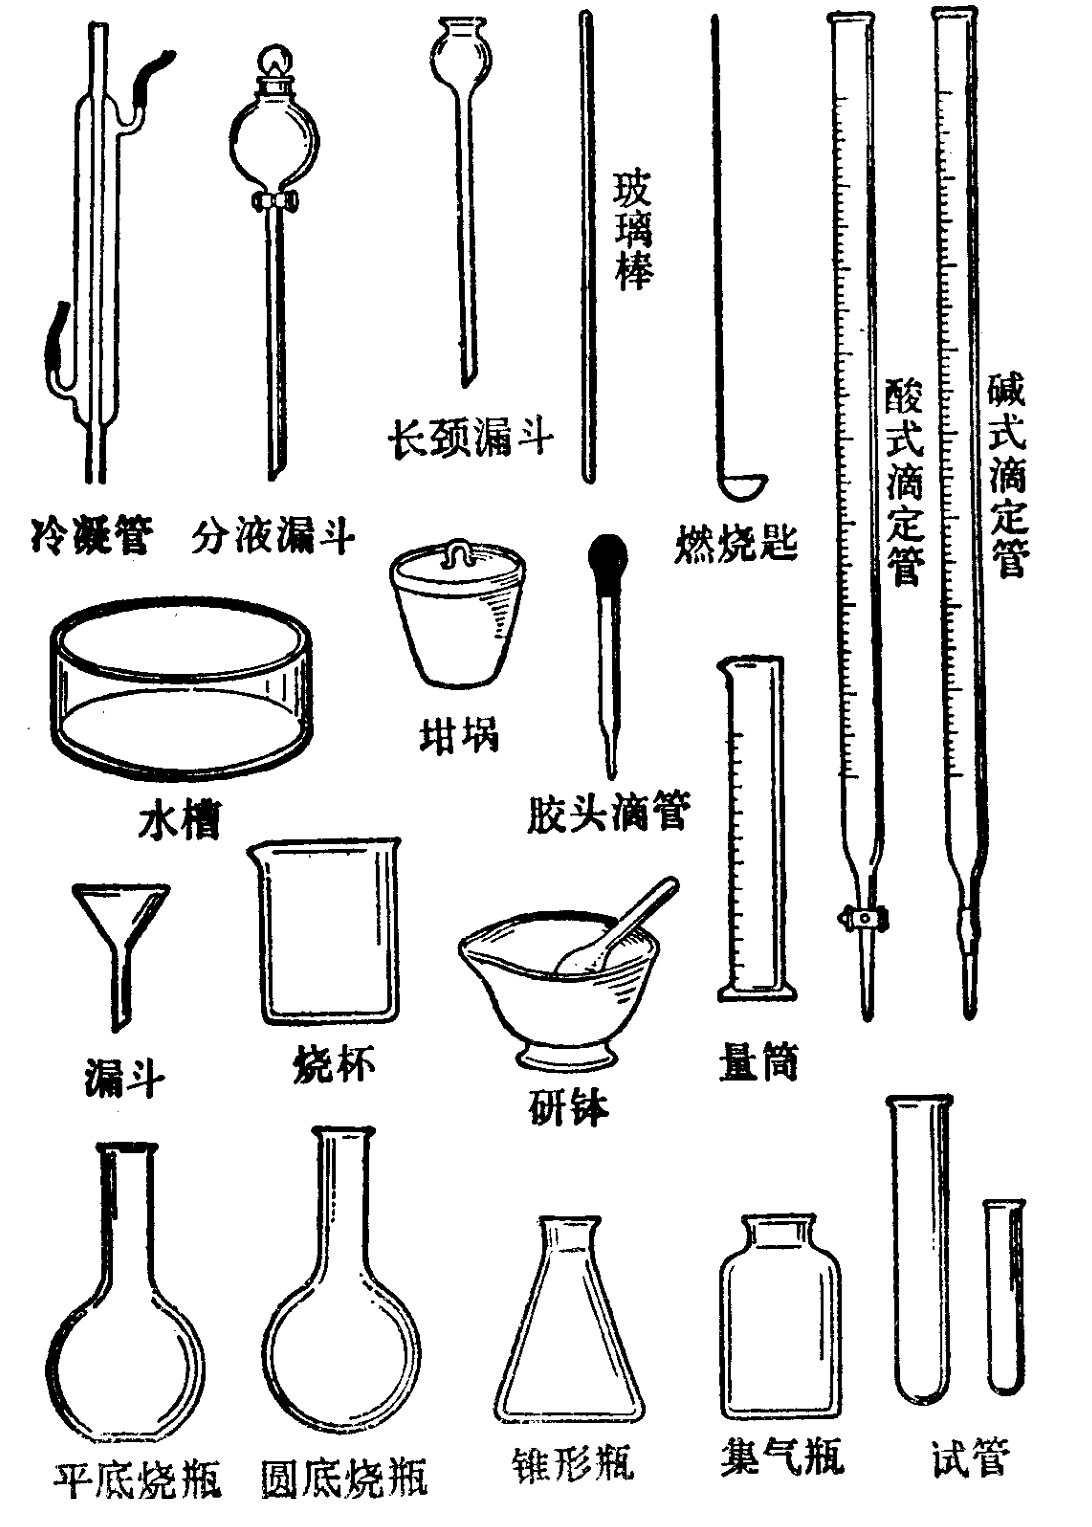
\includegraphics[width=\textwidth]{../pic/czhx1-xssy-yiqi-1.png}
    \caption*{化学实验的常用仪器示意图}
\end{figure}

\begin{figure}[H]
    \centering
    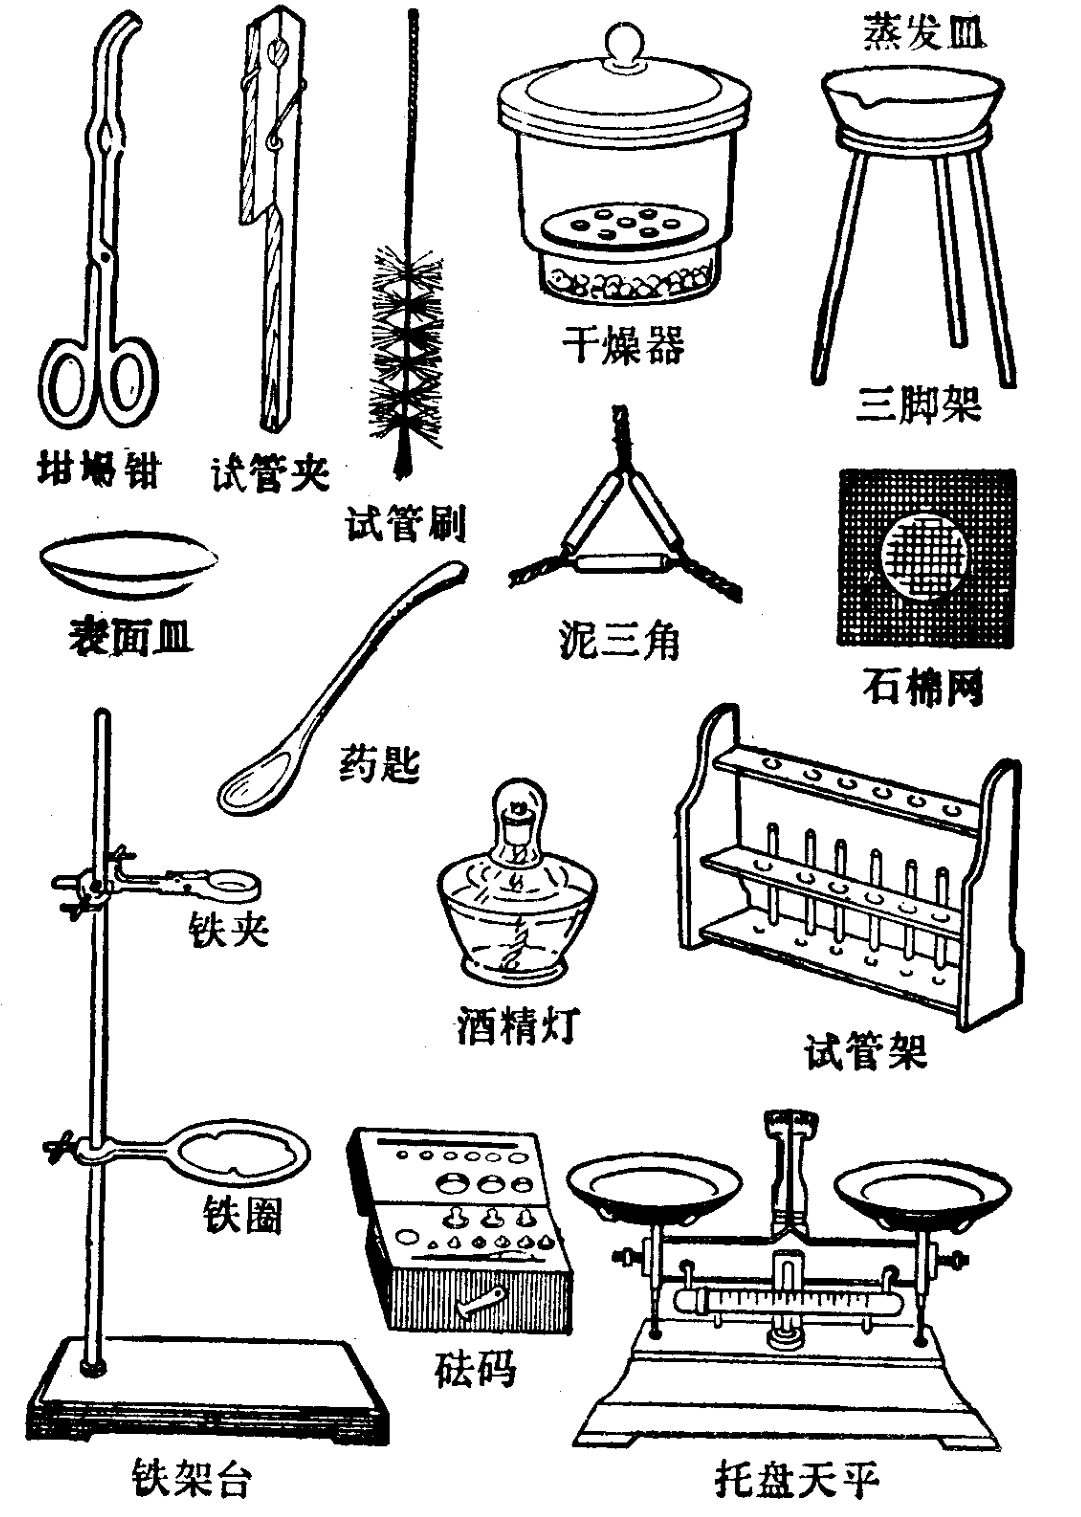
\includegraphics[width=\textwidth]{../pic/czhx1-xssy-yiqi-2.png}
    \caption*{化学实验的常用仪器示意图}
\end{figure}



\begingroup
\renewcommand{\thefigure}{\arabic{figure}\;}
\nonumsection{化学实验基本操作\footnotemark}\label{sec:xssy-caozuo}
\footnotetext{这些基本操作,应先由教师讲解或演示,然后让学生自己练习。教师可根据具体情况采取集中或分散讲解、演示的方法。}

\subsection{药品的取用}

1. 实验里所用的药品,有的有毒性,有的有腐蝕性。
因此,不能用手接触药品,不要把鼻孔凑到容器口去闻气体的气味,\zhongdian{特别注意不得尝药品的味道}。

2. 取用药品,应该严格按照实验说明里规定的用量。
如果实验里没有说明用量,就应该取用最少量:
液体用 1—2 毫升,固体只要盖满试管的底部。

用剩的药品应该交还实验室,不要抛弃, 不要放回原瓶。

3. 固体药品的取用

取用固体药品一般用药匙。药匙的两端为大小两匙,取固体量较多时用大匙,较少时用小匙。
有些块状的药品(如钠、钾、磷块等)可用镊子取用。
用过的药匙或镊子要立刻用干净的纸擦拭干净,以备下次使用。

往试管里装入固体粉末时,为避免药品沾在管口和管壁上,可使试管倾斜,
把盛有药品的药匙(或用小纸条折叠成的纸槽)小心地送入试管底部(图 \ref{fig:xssy-1}),
然后使试管直立起来,让药品全部落到底部。

\begin{figure}[htbp]
    \centering
    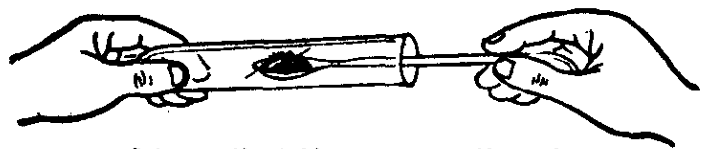
\includegraphics[width=0.6\textwidth]{../pic/czhx1-xssy-01}
    \caption{往试管里送入固体粉末}\label{fig:xssy-1}
\end{figure}

把块状的药品或密度较大的金属颗粒放入玻璃容器时,应该先把容器横放,
把药品或金属颗粒放入容器口以后,再把容器慢慢地竖立起来,
使药品或金属颗粒缓缓地滑到容器的底部,以免打破容器。

\textbf{学生练习}

(1) 用药匙的一端把固体粉末放入一个干燥的试管里(固体粉末可用实验室回收的药品或沙子等物代替)。
再练习把较重的颗粒放入另一个试管里。

(2) 把固体粉末放在折叠成槽状的纸条上,然后送入试管底部(图 \ref{fig:xssy-2} )。


\begin{figure}[htbp]
    \centering
    \begin{minipage}[b]{7cm}
        \centering
        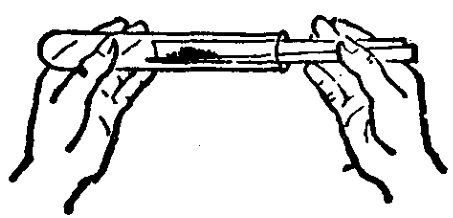
\includegraphics[width=6cm]{../pic/czhx1-xssy-02}
        \caption{用纸槽往试管里送入固体粉末}\label{fig:xssy-2}
    \end{minipage}
    \qquad
    \begin{minipage}[b]{7cm}
        \centering
        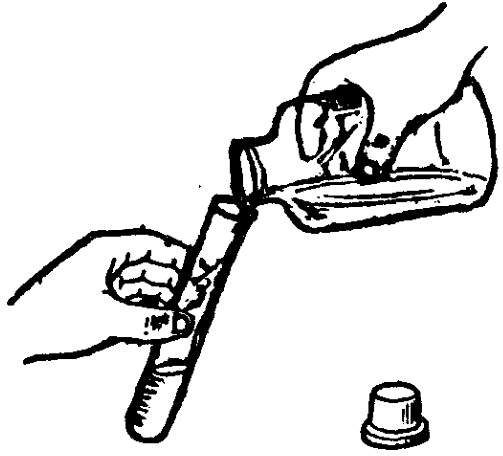
\includegraphics[width=6cm]{../pic/czhx1-xssy-03}
        \caption{液体的倾倒}\label{fig:xssy-3}
    \end{minipage}
\end{figure}


4. 液体药品的取用

液体药品通常盛在细口瓶里。取用的时候,先把瓶塞拿下,倒放在桌上。
然后一手拿起瓶子(瓶上的标签应向着手心,以免倒完药品后,残留在瓶口的药液流下来,腐蚀标签),
另一手略斜地持试管,使瓶口紧挨着试管口(图 \ref{fig:xssy-3} ),把液体缓缓地倒入试管里。

需用液体倒完后,立即盖紧瓶塞,把瓶子放回原处,要注意使瓶上的标签向外。

\textbf{学生练习}

(1) 取一个试管和一个盛有水的细口瓶,按图3 所示练习倾倒液体。

(2) 往三个试管里依次倒入下列容积的水: 1/3 试管, 1/4 试管, 1/5 试管。
要求对每种容积反复练习多次,直到比较熟练为止。


5. 浓酸、浓碱的使用

使用浓酸、浓碱等腐蚀性的药品,必须\zhongdian{特别小心},防止沾到皮肤上或洒在衣服上。

如果酸流到桌上,可以立即往酸里加适量的碳酸氢钠溶液,直到不发生气泡为止。
如果碱溶液流到桌上,可以立即往碱里加适量的稀醋酸来中和。
然后,先用水冲洗桌子,再用抹布擦干净。
如果只有少量酸或碱溶液滴到桌上,可以立即用湿抹布擦净,再用水冲洗抹布。

如果酸沾到皮肤上,立即用较多的水冲洗(皮肤上不慎洒上浓硫酸,不得先用水冲洗,
而要根据情况迅速用布拭去,再用水冲洗), 再涂上 3—5\% 的碳酸氢钠溶液。
如果碱溶液沾到皮肤上,也要用较多的水冲洗,再涂上硼酸溶液。

要注意保护眼睛。万一眼睛里溅进了酸或碱溶液,要立刻用水冲洗(切不可用手揉眼)。
洗的时候要眨眼睛,同时要报告教师,必要时找医生治疗。


\subsection{物质的称量和液体的量取}

1. 托盘天平的使用

托盘天平由托盘(分左右两个)、指针、标尺、调节零点的螺丝、游码、刻度尺等组成(图 \ref{fig:xssy-4})。
托盘天平只能用于粗略的称量,能称准到 $0.1$ 克。

\begin{figure}[htbp]
    \centering
    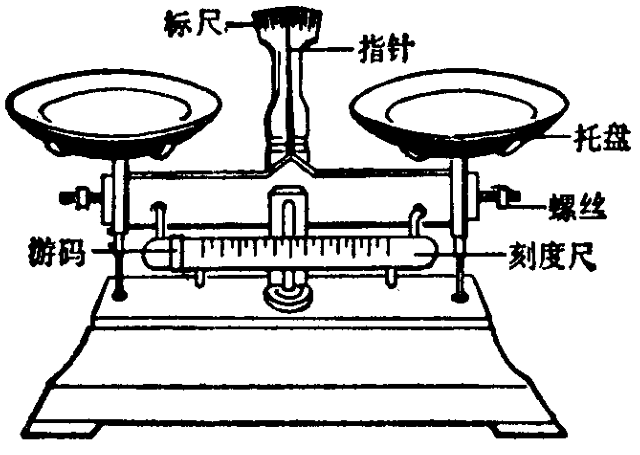
\includegraphics[width=0.5\textwidth]{../pic/czhx1-xssy-04}
    \caption{托盘天平}\label{fig:xssy-4}
\end{figure}

(1) 称量前先把游码放在刻度尺的零处,检查天平的摆动是否到达平衡。
如果已到达平衡,指针摆动时先后指示的标尺上的左、右两边的格数接近相等,指针静止时则应指在标尺的中间。
如果天平的摆动未到达平衡,可以调节左、右的螺丝,使摆动到达平衡。
想一想,如果指针偏向左边,哪一边的托盘的质量较大?应怎样调节螺丝?为什么?

(2) 称量物不能直接放在托盘上。可在两个托盘上各放一张大小相同的同种的纸,然后把要称量的药品放在纸上称量。
潮湿的或具有腐蚀性的药品必须放在玻璃器皿(如表面皿、烧杯)里称量。

(3) 把称量物放在左盘,砝码放在右盘。砝码要用镊子夹取。
先加质量大的砝码,再加质量小的砝码,最后可移动游码,直到天平摆动到达平衡为止。
记录所加砝码和游码的质量。

(4) 称量完毕后,应把砝码放回砝码盒中,把游码移回零处。

\textbf{学生练习}

(1) 把托盘天平放在平坦的桌面上,调节零点。
在天平两边的托盘上各放一张大小相同的同种的纸,观察零点有无变化?
想一想,右托盘上放纸的目的是什么?

(2) 称量 1 药匙食盐(或用沙子等物代替)的质量。记录数据。

(3) 计算 3 药匙食盐的质量。把该质量的砝码放好后再加食盐。
应练习逐渐加食盐到天平摆动到达平衡。
当食盐的量只缺很少时,可用左手拿药匙,右手拍左手手腕,
靠药匙振动而掉下的少量食盐来加足药量。

2. 量筒的使用

取用一定量的液体药品,可用量筒量出体积。量液体时,量筒必须放平稳,
而且使视线与量筒内液体的凹液面的最低处保持水平(图 \ref{fig:xssy-5}),
再读出所取液体的体积数。

\begin{figure}[htbp]
    \centering
    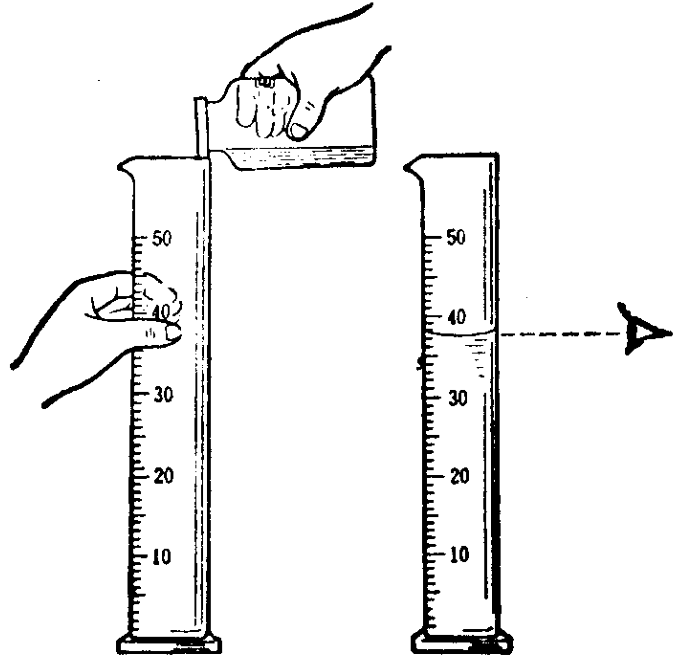
\includegraphics[width=0.5\textwidth]{../pic/czhx1-xssy-05}
    \caption{液体的量取}\label{fig:xssy-5}
\end{figure}


\textbf{学生练习}

(1) 取一个 10 毫升的量筒,把水加到指定容积的刻度( 10 毫升、5 毫升)。反复练习。
当水的量接近所需容积刻度线时,可用一干净滴管取少量水滴入量筒(不要把滴管伸入量筒内或接触筒壁)。

(2) 用 10 毫升的量筒量取 2 毫升的水。把水倒入一个试管里,记住液面在试管里的高度,
然后把试管里的水再倒回 10 毫升的量筒里。用试管再先后 3 次移取约 2 毫升的水到量筒中。
最后读一下量筒中水的体积数。

(3) 用滴管取少量水,向量筒里逐滴加水至 1 毫升,数一数需要多少滴?
再向试管里滴入约 1 毫升水,记住液面在试管里的高度。


\subsection{物质的加热}

1. 使用酒精灯的方法

(1) 使用酒精灯以前,要检查一下灯芯,如果灯芯顶端不平或已烧焦,就要剪去少许;
还要检查灯里有无酒精。向灯里添加酒精,不可超过酒精灯容积的 2/3 。
\zhongdian{绝对禁止向燃着的酒精灯里添加酒精},以免失火。

(2) 为了得到适当大小的火焰,先要调整灯芯,然后用火柴点燃(图 \ref{fig:xssy-6}, I)。
\zhongdian{绝对禁止拿酒精灯到另一已经燃着的酒精灯上去点火}(图 \ref{fig:xssy-6} ,II), \zhongdian{以免失火}。

\begin{figure}[htbp]
    \centering
    \begin{minipage}[b]{4cm}
        \centering
        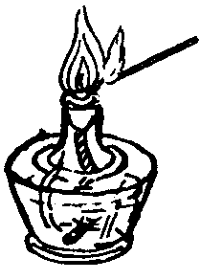
\includegraphics[width=3cm]{../pic/czhx1-xssy-06-1}
        \caption*{I}
    \end{minipage}
    \qquad
    \begin{minipage}[b]{4cm}
        \centering
        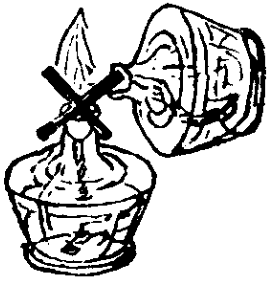
\includegraphics[width=3.5cm]{../pic/czhx1-xssy-06-2}
        \caption*{II}
    \end{minipage}
    \qquad
    \begin{minipage}[b]{4cm}
        \centering
        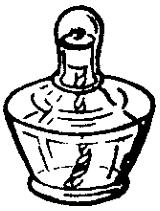
\includegraphics[width=3cm]{../pic/czhx1-xssy-06-3}
        \caption*{III}
    \end{minipage}
    \caption{酒精灯的使用}\label{fig:xssy-6}
\end{figure}

(3) 酒精灯的火焰必须用灯帽盖灭(图 \ref{fig:xssy-6}, III), \zhongdian{不可用嘴吹灭}。
如果用嘴吹,可能引起灯内酒精的燃烧,发生危险。

酒精灯不用的时候,必须盖上灯帽。不然洒精会蒸发掉,这样不但浪费酒精,
而且灯芯上留有水分(商品酒精都含有少量水),以后就不易点燃或燃烧不好。

使用酒精灯要随时小心,不要碰倒。
万一洒出的酒精在桌上燃烧起来,应该立刻用湿抹布扑盖或撒沙土扑灭。

2. 给物质加热

\begin{wrapfigure}[10]{r}{5cm}
    \centering
    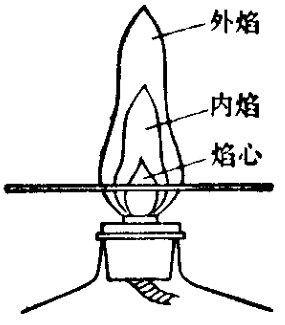
\includegraphics[width=4cm]{../pic/czhx1-xssy-07}
    \caption{酒情灯的灯焰}\label{fig:xssy-7}
\end{wrapfigure}

(1) 酒精灯的火焰可分焰心、内焰、外焰三个部分。
如将一根火柴梗迅速放进酒精灯的火焰中,象图 \ref{fig:xssy-7} 那样平放着。等 1—2 秒钟拿出来,
可以看到处在火焰外层(外焰)的部分最先碳化。
因为外焰燃烧充分,所以外焰温度最高,内焰燃烧不充分,温度较低,焰心温度最低。
加热时,应把受热物质放在外焰部分。


(2) 给液体加热可以用试管、烧瓶、烧杯、蒸发皿;给固体加热可以用干燥的试管、坩埚、烧瓶等。

(3) 给试管里的物质加热,必须使用试管夹。
将试管夹从试管底部往上套,夹在试管的中上部。
用手拿住试管夹的长柄,不要把拇指按在短柄上。
给烧瓶或烧杯里的物质加热,要放在铁架台的铁圈上(烧瓶要用夹子夹住颈部), 垫上石棉网,
使烧瓶或烧杯受热均匀,不致破裂。
用坩埚加热,要把它放在泥三角上。如需移动坩埚,必须用坩埚钳夹住。
用蒸发皿加热,可把它放在铁架台上大小适宜的铁圈上。加热后不要直接用手拿,可使用坩埚钳夹取。

(4) 如果被加热的玻璃容器外壁有水,应在加热前擦拭干净,然后加热,以免容器炸裂。

(5) 加热的时候,不要使玻璃容器的底部跟灯芯接触,以免容器破裂(图 \ref{fig:xssy-8})。
烧得很热的玻璃容器,不要立即用冷水冲洗或放在桌上,否则可能破裂。

\begin{figure}[htbp]
    \centering
    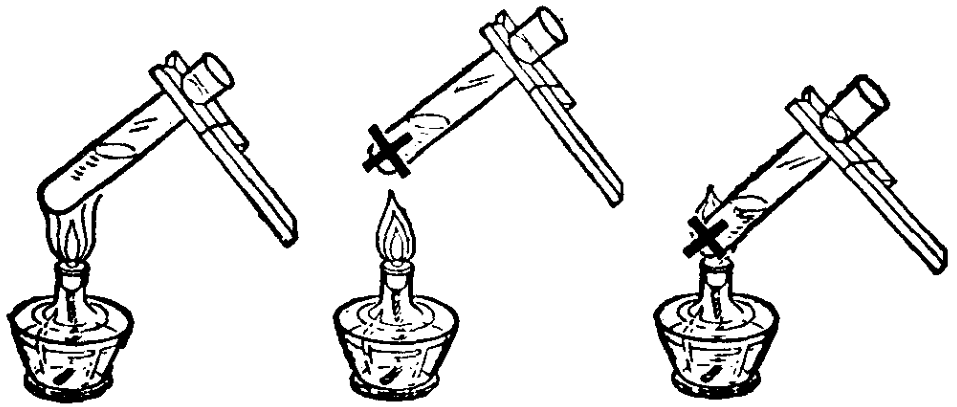
\includegraphics[width=0.7\textwidth]{../pic/czhx1-xssy-08}
    \caption{用酒精灯给物质加热}\label{fig:xssy-8}
\end{figure}


(6) 给试管里的固体加热,应该使试管在火焰上移动(如果试管需要固定,可移动酒精灯),
试管均匀受热后,再将火焰固定在放固体的部分加热。

(7) 给试管里的液体加热,液体体积一般不要超过试管容积的 1/3,
加热时,试管要倾斜(跟桌面成 $45^\circ$ 角)。
先使试管均匀受热,然后小心地在试管里液体的中下部加热,并且不时地上下移动试管。
\zhongdian{为避免试管里液体沸腾喷出伤人,加热时切不可使试管口对着自己或旁人}。

\textbf{学生练习}

(1) 检查一个酒精灯的灯芯和里面的酒精液面是否符合要求。
如不符合要求,请进行调整。
用火柴点燃酒精灯,观察它的火焰,然后熄灭。

(2) 取一个试管,加入 3 毫升的水,用试管夹夹住,按上述要求进行加热。
注意不要使试管口对着自己或别人。
观察在试管底部的某一部分集中加热和不时地上下移动试管加热时,液体沸腾的现象有什么不同。
想一想,为什么要 “不时地上下移动试管”?


\subsection{液体的过滤}

1. 过滤器的准备

取一张圆形滤纸(图 \ref{fig:xssy-9},I), 先折成半圆(图 \ref{fig:xssy-9}, II),再折成四等分(图\ref{fig:xssy-9}, III),
然后打开成圆锥形,把圆锥形的滤纸尖端向下,放入漏斗里,滤纸的边缘应比漏斗口稍低
(大约低 5 毫米,多余的滤纸应该剪去)。然后用手压住,用水润湿,
使滤纸紧贴着漏斗的内壁,中间不要留有气泡(图 \ref{fig:xssy-9}, IV)。
这样就做成一个过滤器。

\begin{figure}[htbp]
    \centering
    \begin{minipage}[b]{3cm}
        \centering
        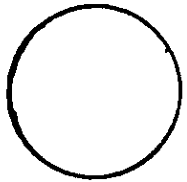
\includegraphics[width=2cm]{../pic/czhx1-xssy-09-1}
        \caption*{I}
    \end{minipage}
    \qquad
    \begin{minipage}[b]{3cm}
        \centering
        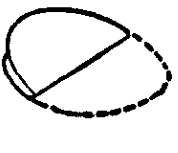
\includegraphics[width=2cm]{../pic/czhx1-xssy-09-2}
        \caption*{II}
    \end{minipage}
    \qquad
    \begin{minipage}[b]{3cm}
        \centering
        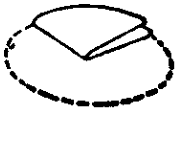
\includegraphics[width=2cm]{../pic/czhx1-xssy-09-3}
        \caption*{III}
    \end{minipage}
    \begin{minipage}[b]{3cm}
        \centering
        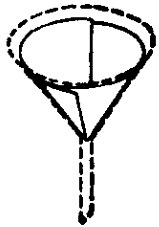
\includegraphics[width=2cm]{../pic/czhx1-xssy-09-4}
        \caption*{IV}
    \end{minipage}
    \caption{过滤器的准备}\label{fig:xssy-9}
\end{figure}


2. 过滤的方法

\begin{wrapfigure}[13]{r}{5cm}
    \centering
    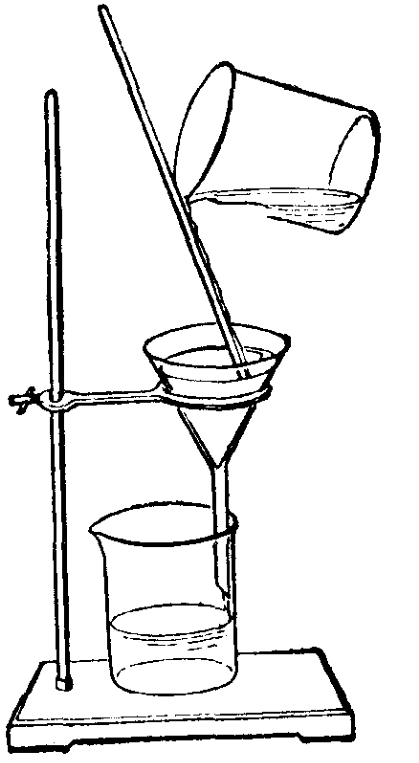
\includegraphics[width=4cm]{../pic/czhx1-xssy-10}
    \caption{过滤的方法}\label{fig:xssy-10}
\end{wrapfigure}

(1) 把过滤器放在铁架台的铁圈(或漏斗架)上,调整高度,
使漏斗下端的管口靠紧烧杯的内壁(图 \ref{fig:xssy-10})。
这样可以使滤液沿烧杯内壁流下,不致溅出来。


(2) 按照图 \ref{fig:xssy-10} 所示,使液体沿着玻璃棒流进过滤器(玻璃棒的末端要轻轻地斜靠在有三层滤纸的一边)。
漏斗里的液体的液面要低于滤纸的边缘,如果液体的液面高于滤纸的边缘,
液体就会从滤纸和漏斗壁之间流下,使固体混入滤液。

(3) 如果滤液仍然浑浊,应该把滤液再过滤一次。

3. 洗涤沉淀的方法

洗涤滤纸上的沉淀,可以照图 \ref{fig:xssy-10} 所示,向漏斗里注入少量水,使水面浸过沉淀物,等水滤出以后,
再次加水洗涤,连洗几次,即可把沉淀洗干净。

\textbf{学生练习}(也可以结合实验一进行)

做一个过滤器。过滤一杯混有泥沙的水。



\subsection{仪器的装配\footnotemark}
\footnotetext{化学实验基本操作五、六的学生练习可结合后面的学生实验进行。}

装配仪器首先要看清楚装置图, 然后选择仪器和零件,一件一件地连接起来,
最后要检查装配好的装置是不是严密不漏气(即检查气密性)。

1. 仪器和零件的连接

(1) 把玻璃管插入带孔像皮塞或软木塞的方法 \quad
左手拿橡皮塞或软木塞,右手拿玻璃管(靠近要插入塞子的一端),
先把玻璃管要插入塞子的一端用水润湿(图 \ref{fig:xssy-11}),
然后稍稍用力转动(小心!不要使玻璃管折断,以致刺破手掌),使它插入。


\begin{figure}[htbp]
    \centering
    \begin{minipage}[b]{7cm}
        \centering
        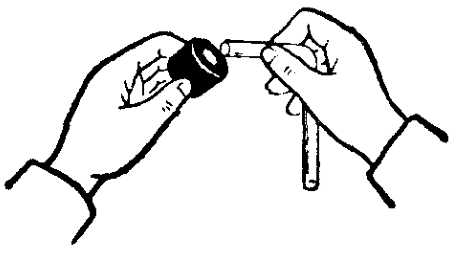
\includegraphics[width=5cm]{../pic/czhx1-xssy-11}
        \caption{把坡璃管插入橡皮塞的孔里}\label{fig:xssy-11}
    \end{minipage}
    \qquad
    \begin{minipage}[b]{7cm}
        \centering
        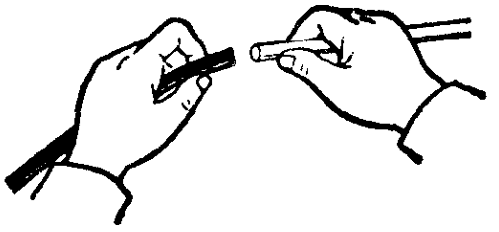
\includegraphics[width=5cm]{../pic/czhx1-xssy-12}
        \caption{在玻璃管上套上橡皮管}\label{fig:xssy-12}
    \end{minipage}
\end{figure}

(2) 使玻璃管跟橡皮管连接的方法 \quad 左手拿橡皮管,
右手拿玻璃管(图 \ref{fig:xssy-12}), 先把玻璃管口用水润湿,稍稍用力把玻璃管插入橡皮管。

\begin{wrapfigure}[8]{r}{6cm}
    \centering
    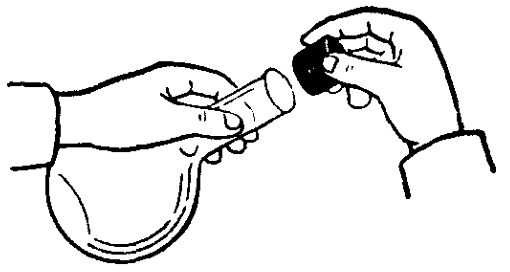
\includegraphics[width=5cm]{../pic/czhx1-xssy-13}
    \caption{用橡皮塞塞住烧瓶}\label{fig:xssy-13}
\end{wrapfigure}

(3) 在烧瓶口塞橡皮塞的方法 \quad 左手拿烧瓶颈,右手拿橡皮塞慢慢转动,塞进瓶口(图 \ref{fig:xssy-13})。
切不可把烧瓶放在桌上再使劲塞进塞子。因为这样做容易压破烧瓶。
在试管口塞橡皮塞,也要用同样的方法。


2. 装置的气密性的检查

要检查图 \ref{fig:xssy-14} 的装置是不是漏气,可以把导管的一端浸入水里,用手掌紧贴烧瓶的外壁。
如果装置不漏气,烧瓶里的空气受热膨胀,导管口就有气泡冒出(图 \ref{fig:xssy-14},I)。
把手移开,过一会儿烧瓶冷却,水就升到导管里,形成一段水柱(图 \ref{fig:xssy-14},II)。

\begin{figure}[htbp]
    \centering
    \begin{minipage}[b]{7cm}
        \centering
        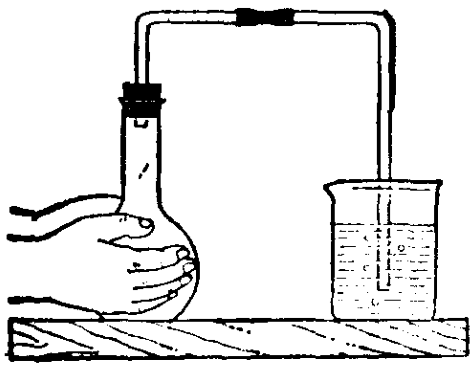
\includegraphics[width=5cm]{../pic/czhx1-xssy-14-1}
        \caption*{I}
    \end{minipage}
    \qquad
    \begin{minipage}[b]{7cm}
        \centering
        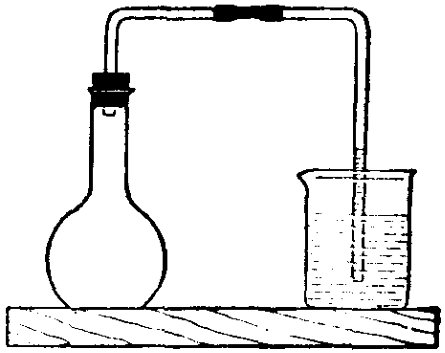
\includegraphics[width=5cm]{../pic/czhx1-xssy-14-2}
        \caption*{II}
    \end{minipage}
    \caption{检验装置的气密性}\label{fig:xssy-14}
\end{figure}

如果发现装置漏气,必须找出漏气的原因,并进行调整、修理,或更换零件。



\subsection{玻璃仪器的洗涤}

做实验必须用干净的玻璃仪器,否则会影响实验的效果。

做完实验,应该立刻把用过的玻璃仪器洗刷干净。

洗涤试管或烧瓶,可以注入半管或半瓶水,稍稍用力振荡,把水倒掉(图 \ref{fig:xssy-15}),照这样连洗数次。
如果内壁附有不易洗掉的物质,可以用试管刷刷洗。
刷洗时,使试管刷在盛水的试管里转动或上下移动,但用力不能过猛,否则容易把试管底弄破。


\begin{figure}[htbp]
    \centering
    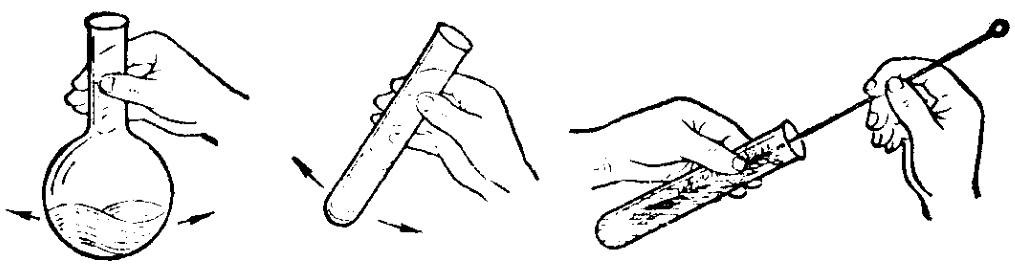
\includegraphics[width=0.7\textwidth]{../pic/czhx1-xssy-15}
    \caption{玻璃仪器的洗涤}\label{fig:xssy-15}
\end{figure}

玻璃仪器里如附有不溶于水的碱、碳酸盐、碱性氧化物等物质,可以先加稀盐酸溶解,再用水冲洗。
玻璃仪器里如附有油脂,可以先用热的纯碱(碳酸钠)溶液洗,再用试管刷刷洗,
也可用试管刷蘸少量去污粉或洗衣粉刷洗,然后用水把试管冲洗干净。

玻璃仪器洗过以后,如果内壁上附着的水均匀了,既不聚成水滴,也不成股流下,这才算洗干净了。

洗干净的玻璃仪器,应该倒放在平稳的地方,或放在试管架上晾干。

实验完毕,导管、橡皮塞等其它零件,也要用水洗干净。




\ctexset {
    section={
        name={实验,},
        number=\chinese{section},
    },
}
\newenvironment{shiyanmudi}{
    \textbf{实验目的} 
}{}
\newenvironment{shiyanyongpin}{
    \textbf{实验用品} 
}{}
\newenvironment{shiyanbuzhou}{
    \textbf{实验步骤} \par
}{}
\newenvironment{wentihetaolun}{
    \textbf{问题和讨论} \par
}{}
\newenvironment{shiyanxiti}{
    \textbf{实验习题} \par
}{}

\section{粗盐的提纯}\label{sec:xssy-sy1}

\begin{shiyanmudi}
    初步学会溶解、过滤和蒸发等基本操作。
\end{shiyanmudi}

\begin{shiyanyongpin}
    烧杯、玻璃棒、蒸发皿、酒精灯、漏斗、药匙、量筒(10 毫升)、铁架台(带铁圈)、滤纸、剪刀、托盘天平。

    粗盐。
\end{shiyanyongpin}

\begin{shiyanbuzhou}
    1. 粗盐的溶解 在天平上称取 5 克粗盐(精确至 $0.1$ 克)放在桌上备用。

    \begin{wrapfigure}[16]{r}{5cm}
        \centering
        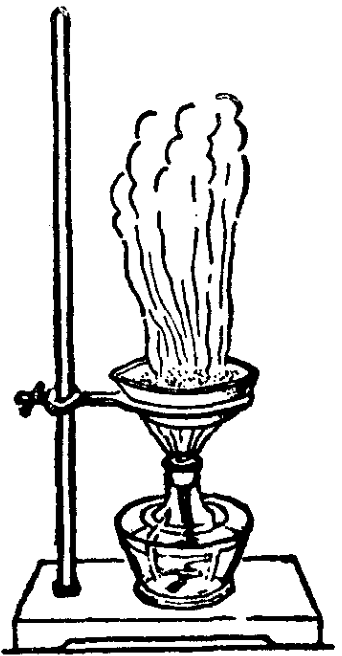
\includegraphics[width=4cm]{../pic/czhx1-xssy-16}
        \caption{蒸发}\label{fig:xssy-16}
    \end{wrapfigure}

    用量筒量取 10 毫升水倒入烧杯里。用药匙取一匙粗盐加入水中,先不搅拌水,观察发生的现象。
    再用玻璃棒搅拌,并观察发生的现象。玻璃棒的搅拌对粗盐的溶解起什么作用?
    接着再加入粗盐,边加边用玻璃棒搅拌,一直加到粗盐不能溶解为止。观察食盐水是否浑浊。

    在天平上称量剩余的粗盐。计算一下在 10 毫升水中约溶解粗盐多少克?

    2. 过滤 按照实验基本操作四所述的方法做一个过滤器,用来过滤食盐水(注意玻璃棒的使用方法)。
    等过滤完毕后,观察滤纸上剩余的物质及滤液的颜色和状态。
    如果滤液还浑浊,应该再过滤一次。观察滤液是否透明。

    3. 滤液的蒸发 把透明的滤液倒入蒸发皿里,再把蒸发皿放在铁架台的铁圈上,用酒精灯加热(图 \ref{fig:xssy-16})。

    在加热过程中,要用玻璃棒不断搅拌液体,以免液体局部过热,致使液滴飞溅出来。
    等到蒸发皿中出现多量固体时,就停止加热。

    4. 固体食盐的洗涤 用玻璃棒把固体移入一个新做的过滤器里,用少量水均匀冲洗,洗掉固体表面残留的液体。

    把制得的食盐跟原来的粗盐进行比较,然后把食盐倒在教师指定的容器里。
\end{shiyanbuzhou}

\begin{wentihetaolun}

    1. 根据实验中得到的数据,估算在 100 毫升水中约能溶解粗盐多少克?

    2. 在这个实验里有几个使用玻璃棒的操作,在各个操作中,玻璃棒起的作用有什么不同?

    3. 在进行过滤时要注意哪几点?为什么?

\end{wentihetaolun}

\section{制取蒸馏水}\label{sec:xssy-sy2}

\begin{shiyanmudi}
    1. 学习仪器装配的操作; 2. 学习蒸馏的操作。
\end{shiyanmudi}

\begin{shiyanyongpin}
    圆底烧瓶、导管、橡皮管、单孔橡皮塞、胶头滴管、试管、烧杯、酒精灯、铁架台(带铁圈和铁夹)、石棉网。

    高锰酸钾溶液。
\end{shiyanyongpin}

\begin{shiyanbuzhou}

    \begin{wrapfigure}[16]{r}{7cm}
        \centering
        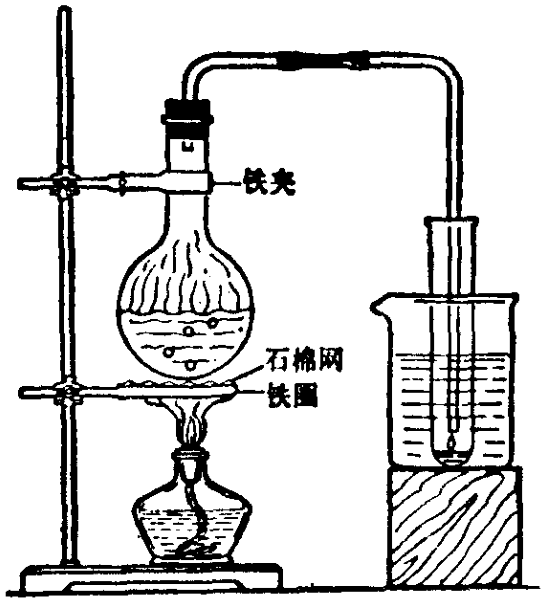
\includegraphics[width=6cm]{../pic/czhx1-xssy-17}
        \caption{制取蒸馏水的装置}\label{fig:xssy-17}
    \end{wrapfigure}

    1. 按化学实验基本操作五中仪器装配的要求,把烧瓶和导管连接好,并检查气密性。
    在烧瓶里倒入半瓶热水,用滴管取少量高锰酸钾溶液(观察它的颜色),
    把这种溶液滴入烧瓶里几滴,观察烧瓶里溶液的颜色。

    2. 按图 \ref{fig:xssy-17} 安装好仪器(注意酒精灯、铁圈和铁夹放置的位置)。
    烧杯中放入用来冷凝水蒸气的冷水。导管的末端应该跟试管底相距 2—3 厘米。
    为什么之必须保持这一段距离?

    3. 装置全部连接好以后,用酒精灯加热。加热的时候,注意不要使烧瓶里的液体沸腾得太厉害。
    如果沸腾得太厉害,液体就会直接通过导管流到试管里去(可以加几片碎瓷片,以防暴沸)。

    4. 观察蒸馏水的生成。用开始收集到的 2—3 毫升蒸馏水洗涤试管壁,倒掉。
    再用该试管收集 2—3 毫升蒸馏水,然后把导管从试管中取出,停止加热,取出试管。

    观察制得的蒸馏水的颜色,并与烧瓶里的液体颜色作比较。
\end{shiyanbuzhou}

\begin{wentihetaolun}

    1. 说出制得的蒸馏水的颜色,起初滴加的高锰酸钾最后残留在哪里?由此说明蒸馏的作用。

    2. 分别说出实验中使用的石棉网、铁夹和铁圈的作用。

\end{wentihetaolun}


\section{氧气的制取和性质}\label{sec:xssy-sy3}

\begin{shiyanmudi}
    1. 学会实验室制氧气的方法,并试验氧气的性质; 2. 学会用排水法收集气体。
\end{shiyanmudi}


\begin{shiyanyongpin}
    大试管、试管夹、单孔橡皮塞、橡皮管、导管、集气瓶(125 毫升)、水槽、铁架台(带铁夹)、坩埚钳、酒精灯、玻璃片、燃烧匙、木条。

    氯酸钾、二氧化锰、高锰酸钾、木炭、红磷、棉花、石灰水。
\end{shiyanyongpin}

\begin{shiyanbuzhou}
    1. 二氧化锰对氯酸钾分解的催化作用

    观察氯酸钾和二氧化锰的颜色、状态。

    在一洁净\footnote{做这个实验,试管必须洁净,特别是管壁上不能附着有机物杂质,否则容易发生爆炸,造成事故。}
    而干燥的试管里加入约 $0.5$ 克氯酸钾,用试管夹夹住试管进行加热,使氯酸钾熔化。取带火星的木条伸入试管。
    观察发生的现象。这时候有没有氧气放出?把试管撤离火焰,撒入少量二氧化锰粉末,立即把准备好的带火星的木条伸入管内。
    观察到什么现象?从这个实验得出什么结论?

    2. 用加热分解高锰酸钾的方法制取氧气

    观察高锰酸钾的颜色和状态。

    用带有导管的橡皮塞塞紧试管。检查这个装置是否漏气。
    拔开橡皮塞,在上述试管里放进大约 7 克的高锰酸钾。
    用一团棉花放在靠近试管口的地方,以防止加热时高锰酸钾粉末进入导管。
    然后把带有导管的塞子塞紧试管口。

    用铁夹把这个装置固定在铁架台上(图 \ref{fig:xssy-18})。将集气瓶盛满水,并用玻璃片盖住瓶口%
    \footnote{用玻璃片盖瓶口时,可以先盖住一小部分,随后推动玻璃片.直至把瓶口全部盖住。}
    (注意不要让瓶口水面留有气泡)。把盛满水的瓶子连同玻璃片一起倒立在盛水的水槽内。
    观察瓶底有没有气泡。如果有气泡,就要重新操作。

    \begin{figure}[htbp]
        \centering
        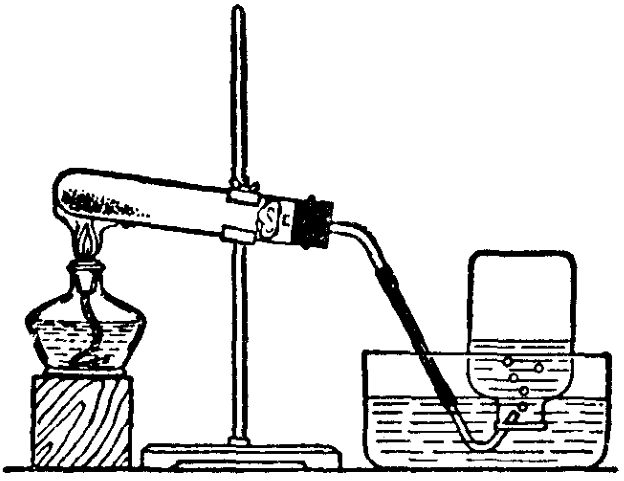
\includegraphics[width=0.5\textwidth]{../pic/czhx1-xssy-18}
        \caption{实验室制取氧气}\label{fig:xssy-18}
    \end{figure}


    给试管加热。先使酒精灯在试管下方来回移动,让试管均匀受热,然后对高锰酸钾所在的部位加热。

    导管口开始有气泡放出时,不宜立即收集,为什么?
    当气泡连续地并比较均匀地放出后,再把导管口伸入盛满水的集气瓶里。
    等瓶子里的水排完以后,(你怎样判断?)用玻璃片盖住瓶口。
    小心地把瓶子移出水槽,正放在桌子上。用同样的方法再收集一瓶氧气。
    停止加热时,先要把导管移出水面,然后熄灭火焰,为什么?

    观察收集到的氧气的颜色,并用带有火星的木条插入集气瓶口检验氧气的存在
    (检验后立即用玻璃片盖住集气瓶口,使瓶里剩余的氧气足够供下面的实验用)。
    记录观察到的现象。

    3. 试验氧气的化学性质

    (1) 木炭在氧气里燃烧 \quad 用坩埚钳夹取一小块木炭在酒精灯的火焰上烧到发红,放在燃烧匙里,立刻插入盛有氧气的集气里。
    观察有什么现象发生。燃烧停止后,取出燃烧匙,往集气瓶里加入少量澄清石灰水,再振荡一下。有什么现象发生?
    木炭在氧气里燃烧,生成什么物质?

    (2) 磷在氧气里燃烧 \quad 取少量红磷放在燃烧匙里,在酒精灯火焰上燃着,注意观察磷在空气里燃烧的情况,
    然后赶快把燃烧匙插入另一盛满氧气的集气瓶里,并立即将玻璃片盖上,观察有什么现象发生。
    比较磷在空气里燃烧和在氧气里燃烧的情况。注意磷燃烧时产生浓厚的白烟,这是五氧化二磷的粉末。
\end{shiyanbuzhou}

\begin{wentihetaolun}

    1. 根据课堂实验和上面的实验,总结氧气的物理性质和化学性质,并填入下表。

    \begin{table}[H]
        \hspace*{4em}\begin{tblr}{
            rowsep=0pt,
            row{1}={abovesep=0.5em, belowsep=0.5em},
            hline{1,8}={1.5pt,solid},
            hline{2}={solid},
            vline{1,5}={1.5pt,solid},
            vline{3}={solid},
            column{2}={6em},
            column{4}={12em},
        }
            \SetCell[c=2]{c}物理性质 & & \SetCell[c=2]{c}化学性质 & \\
            状态(通常情况下)& \xhx[5em] & (1) & 氧气跟非金属反应 \\
            颜色             & \xhx[5em] &     &  \ce{\text{碳} + \text{氧气} ->} \\
            气味             & \xhx[5em] &     &  \ce{\text{硫} + \text{氧气} ->} \\
            密度(跟空气比较)& \xhx[5em] &     &  \ce{\text{磷} + \text{氧气} ->} \\
            溶解性(对水)    & \xhx[5em] & (2) &  氧气跟金属反应 \\
                             &           &    &  \ce{\text{铁} + \text{氧气} ->}
        \end{tblr}
    \end{table}

    2. 收集氧气能不能用向上排空气法?为什么?如果改用向上排空气法收集氧气,实验用品需作什么改动?

    3. 在实验步骤 1、2 中,应根据什么调节试管的高度?

\end{wentihetaolun}


\section{氢气的制取和性质}\label{sec:xssy-sy4}

\begin{shiyanmudi}
    1. 学会实验室制取氢气和检验氢气纯度的方法; 2. 试验氢气的重要化学性质。
\end{shiyanmudi}


\begin{shiyanyongpin}
    试管、烧杯、酒精灯、铁架台(带铁夹)、单孔橡皮塞、导管、橡皮管、水槽。

    锌粒、稀硫酸($1:4$)\footnote{稀硫酸 ($1:4$)指的是 1 体积浓酸跟 4 体积蒸馏水混和而配成的溶液。}、氧化铜。
\end{shiyanyongpin}


\begin{shiyanbuzhou}
    1. 制取氢气和检验氢气的纯度

    (1) 照图 \ref{fig:xssy-19} 那样把发生氢气的装置连接好,检查这个装置的气密性。

    \begin{figure}[htbp]
        \centering
        \begin{minipage}[b]{7cm}
            \centering
            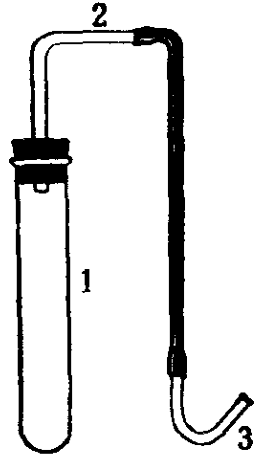
\includegraphics[width=2.8cm]{../pic/czhx1-xssy-19}
            \caption{制取氢气的简单装置}\label{fig:xssy-19}
        \end{minipage}
        \qquad
        \begin{minipage}[b]{7cm}
            \centering
            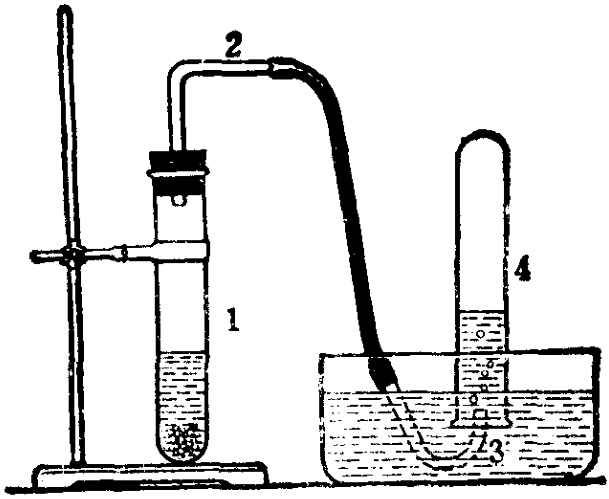
\includegraphics[width=6cm]{../pic/czhx1-xssy-20}
            \caption{制取氢气}\label{fig:xssy-20}
        \end{minipage}
    \end{figure}

    (2) 试管 1 里放入锌粒约 4 克,并注入稀硫酸(占试管 1 容积的 1/3)。
    立即用带有导管 2 的橡皮塞塞住管口,并把这个试管固定在铁架台上。

    锌粒跟稀硫酸接触后,可观察到什么现象?写出这个反应的化学方程式。

    (3) 将试管 4 装满水,用大拇指堵住管口,使管口向下,放入水中,然后照图 \ref{fig:xssy-20} 那样将导管 3 插入试管 4 里收集气体。
    当试管已集满气体时,用右手拿管底,管口朝下,一拿出水面,立即移近酒精灯火焰,点燃试管里的气体,如果听见尖锐的爆鸣声,这证明了什么?
    继续用同样方法收集另一试管气体进行试验,直到听到 “噗” 的声音,证明试管里收集到的氢气已经纯净时为止。

    2. 试验氢气的重要化学性质

    (1) 氢气的可燃性

    如果经过检验,确切地知道从装置里出来的氢气是纯净的,就可以把导管移出水面,用燃着的火柴把氢气点燃。
    观察氢气燃烧时的火焰。用干冷的小烧杯罩在氢气的火焰上(图 \ref{fig:xssy-21}),观察烧杯内壁上发生的现象,写出氢气燃烧的化学方程式。

    \begin{figure}[htbp]
        \centering
        \begin{minipage}[b]{7cm}
            \centering
            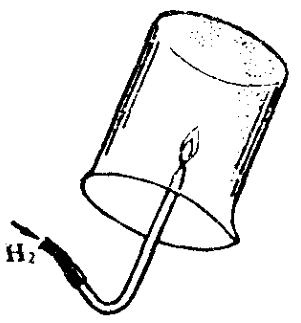
\includegraphics[width=4cm]{../pic/czhx1-xssy-21}
            \caption{氢气的可燃性}\label{fig:xssy-21}
        \end{minipage}
        \qquad
        \begin{minipage}[b]{7cm}
            \centering
            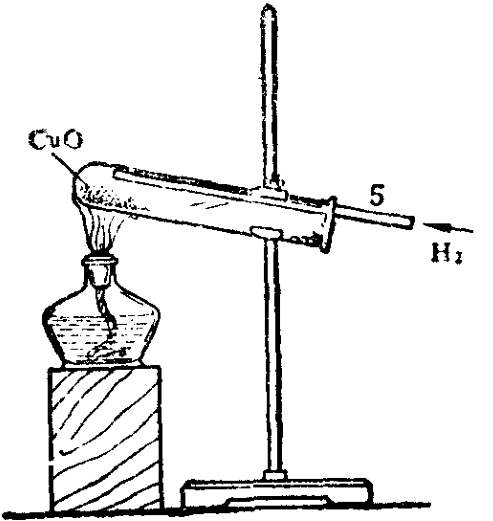
\includegraphics[width=6cm]{../pic/czhx1-xssy-22}
            \caption{氢气还原氧化铜}\label{fig:xssy-22}
        \end{minipage}
    \end{figure}

    (2) 氢气的还原性

    取少量氧化铜铺在干燥的试管的底部,按图 \ref{fig:xssy-22} 装置好。把导管 3 换成直导管 5。注意把试管口稍略微向下倾斜。
    通入经检验已证明是纯净的氢气,大约过一分钟,再加热试管里铺有氧化铜的部位。观察试管里发生的现象,写出这个反应的化学方程式。
\end{shiyanbuzhou}


\begin{wentihetaolun}
    1. 根据上面所做的实验,叙述氢气的物理性质和化学性质。

    2. 根据氢气的性质,可以采用哪些方法收集氢气?

    3. 点燃氢气前,为什么要检验氢气的纯度?怎样检验?

    4. 做氢气的还原性实验时,当氢气刚通入盛有氧化铜的试管时,能不能立即给试管加热?为什么?
\end{wentihetaolun}


\section{二氧化碳的制取和性质}\label{sec:xssy-sy5}

\begin{shiyanmudi}
    1. 学会二氧化碳的实验室制法和用向上排空气法收集气体; 2. 试验二氧化碳的性质。
\end{shiyanmudi}


\begin{shiyanyongpin}
    烧杯、集气瓶、量筒、平底烧瓶、导管、橡皮管、单孔橡皮塞、铁架、试管、试管夹、玻璃片、酒精灯、蜡烛、木条。

    碳酸钙、稀盐酸($1:2$)、石灰水、石蕊试液、蒸馏水。
\end{shiyanyongpin}


\begin{shiyanbuzhou}
    1. 制取二氧化碳

    (1) 按照图 \ref{fig:xssy-23} 那样把装置连接好。检查这个装置的气密性。

    \begin{figure}[htbp]
        \centering
        \begin{minipage}[b]{7cm}
            \centering
            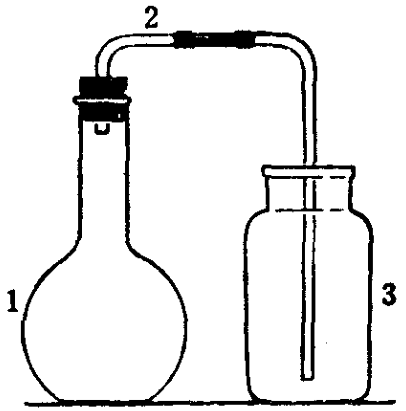
\includegraphics[width=5cm]{../pic/czhx1-xssy-23}
            \caption{制取二氧化碳的装置}\label{fig:xssy-23}
        \end{minipage}
        \qquad
        \begin{minipage}[b]{7cm}
            \centering
            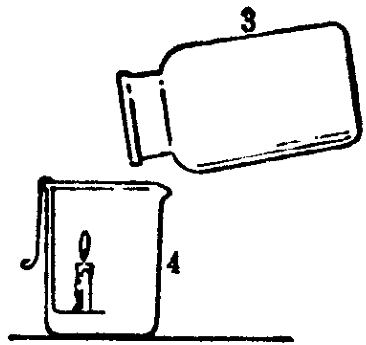
\includegraphics[width=5cm]{../pic/czhx1-xssy-24}
            \caption{把二氧化碳倒入燃着蜡烛的烧杯里}\label{fig:xssy-24}
        \end{minipage}
    \end{figure}

    (2) 在平底烧瓶 1 里放入几小块碳酸钙(想一想应该怎么放)。然后小心地注入稀盐酸 15 毫升。
    立即用带有导管 2 的橡皮塞塞住瓶口,观察烧瓶里发生的现象以及反应中产生气体的颜色。
    过一会儿,可用燃着的木条检查集气瓶 3 里是不是已集满二氧化碳(检查时,木条应放在瓶口还是伸入瓶内)。
    用玻璃片盖住已集满二氧化碳的集气瓶。记录实验现象,并写出有关反应的化学方程式。

    2. 试验二氧化碳的性质

    (1) 把一支短蜡烛固定在烧杯 4 的铁架上,用火点着。
    拿起集满二氧化碳的集气瓶 3,象倒水一样,把二氧化碳倒入烧杯 4 里(图 \ref{fig:xssy-24})。
    观察有什么现象发生。这个实验证明二氧化碳具有什么性质?

    (2) 在一个试管里注入少量澄清的石灰水,通入二氧化碳,发生什么现象?
    继续通入二氧化碳,又有什么现象发生?如果试管里的液体变得澄清,用试管夹夹住试管进行加热,又有什么现象发生?
    解释这一系列变化的原因,并写出这些反应的化学方程式。

    如果从实验步骤 1 制得的二氧化碳的量,不足以供继续实验用,可以把烧瓶 1 里的残留物倒掉,
    另加入几小块碳酸钙和 10—15 毫升稀盐酸,重新制取二氧化碳。

    (3) 在一个试管里加入 2 毫升蒸馏水,滴入 1—2 滴石蕊试液,观察溶液的颜色。
    通入二氧化碳,再观察溶液的颜色有没有变化? 为什么?
\end{shiyanbuzhou}


\begin{wentihetaolun}
    1. 通过以上实验,证明二氧化碳有哪些物理性质和化学性质?

    2. 用排水法和排空气法(又分向上和向下两种)收集气体,分别根据气体的什么性质?
    如要收集氧气、氢气和二氧化碳气体,可分别用什么方法?

    3. 有四瓶无色气体,分别是空气、氢气、氧气和二氧化碳。怎样鉴别它们?叙述操作过程和可能观察到的现象。

    4. 怎样证明鸡蛋壳和锅炉水垢里的主要成分是碳酸钙?
\end{wentihetaolun}


\section{配制一定浓度的溶液}\label{sec:xssy-sy6}

\begin{shiyanmudi}
    1. 学会配制一定质量百分比浓度的溶液; 2. 学会配制一定体积比浓度的溶液。
\end{shiyanmudi}


\begin{shiyanyongpin}
    托盘天平、烧杯、玻璃棒、药匙、量筒(100 毫升、10 毫升)。

    氯化钠、浓盐酸(密度是 $1.19 \; \kmlflm$)。
\end{shiyanyongpin}


\begin{shiyanbuzhou}
    1. 氯化钠溶液的配制

    (1) 计算 \quad 配制 50 克 $5\%$ 的氯化钠溶液,需要氯化钠 \xhx 克和水 \xhx 克。

    (2) 称量 \quad 按托盘天平的使用要求进行称量操作,称量所需的氯化钠,倒入烧杯里。

    (3) 溶解 \quad 水在 4 ℃ 时的密度为 $1 \; \kmlflm$。用量筒量取 \xhx 毫升水,即可近似地看作是 \xhx 克水。
    把量取好的水倒入装有氯化钠的烧杯里,用玻璃棒搅拌,使氯化钠溶解。这样可以制得 50 克 $5\%$ 的氯化钠溶液。

    2. 稀盐酸的配制

    (1) 计算 \quad 用 5 毫升浓盐酸配制 $1:4$ 的稀盐酸,需加水 \xhx 毫升。

    (2) 量取 \quad 用 10 毫升的量筒量取 5 毫升浓盐酸,把浓盐酸倒入烧杯里。

    (3) 溶解 \quad 用量筒量取所需加的水,把水倒入盛有盐酸的烧杯里,边加边搅拌,使盐酸和水混和均匀。
\end{shiyanbuzhou}


\begin{wentihetaolun}
    1. 在实验步骤 1 中,为什么可以不直接用天平称量水的质量,而换算成体积,用量筒量取?

    2. 在实验步骤 2 中,为什么不选用 100 毫升的量筒量取 5 毫升浓盐酸?
\end{wentihetaolun}


\section{酸的性质}\label{sec:xssy-sy7}

\begin{shiyanmudi}
    巩固和加深对酸的性质的认识。
\end{shiyanmudi}


\begin{shiyanyongpin}
    试管、试管夹、药匙、酒精灯、玻璃棒、pH 试纸。

    稀盐酸($1:4$)、稀硫酸($1:4$)、稀硝酸($1:4$)、铁片、锌粒、铜片、氧化铜、带锈铁钉、
    氯化钡溶液、硝酸银溶液、碳酸钠、氢氧化钙、石蕊试液、酚酞试液。
\end{shiyanyongpin}


\begin{shiyanbuzhou}
    1. 酸对指示剂的作用

    (1) 在三个试管里分别倒入稀盐酸、稀硫酸和稀硝酸各 2 毫升。观察颜色、状态,并闻气味。
    在每个试管里放入一根玻璃棒。分别用玻璃棒沾一滴酸液到 pH 试纸上。观察试纸颜色的变化
    (显色以半分钟内的变化为准),跟比色卡对比,测出这三种酸的 pH 值。

    (2) 把玻璃棒从上面三个试管里取出,分别滴入 1—2 滴石蕊试液,振荡。观察发生的现象。

    (3) 在三个试管里分别倒入稀盐酸、稀硫酸和稀硝酸各 2 毫升, 分别滴入 1—2 滴酚酞试液, 振荡。观察发生的现象。

    2. 酸跟金属的反应

    在三个试管里分别加入稀盐酸各 2 毫升,依次把铁片、锌粒和铜片放在试管里,观察发生的现象。
    把燃着的火柴移近有现象发生的试管口,又发生什么现象?写出反应的化学方程式,并解释为什么有的试管里没有什么现象发生。

    3. 酸跟碱性氧化物的反应

    (1) 用药匙向一干燥的试管里加入少量氧化铜。然后再向试管里倒入 2 毫升稀硫酸,小心地加热试管
    (注意不要使稀硫酸沸腾),并轻轻振荡。观察发生的现象。写出反应的化学方程式。

    (2) 取一根带锈的铁钉,轻轻地放入试管(应该怎么放)。倒入 2 毫升稀盐酸,加热,直到铁钉上的锈
    (主要成分是 \ce{Fe2O3.H2O}) 去掉为止。写出反应的化学方程式。

    4. 酸跟盐的反应

    (1) 在试管里加入 2 毫升稀硫酸,再滴入几滴氯化钡溶液。观察发生的现象。写出反应的化学方程式。

    (2) 在试管里加入 2 毫升稀盐酸,再滴入几滴硝酸银溶液。观察发生的现象。写出反应的化学方程式。

    (3) 在试管里加入少量碳酸钠粉末,再滴入几滴稀盐酸。观察发生的现象。写出反应的化学方程式。

    5. 酸跟碱的反应

    在试管里加入少量氢氧化钙粉末,再加入少量稀盐酸。观察发生的现象。写出反应的化学方程式。
\end{shiyanbuzhou}


\begin{wentihetaolun}
    1. 根据实验说明检验一种溶液是不是酸溶液,可以用什么方法?

    2. 根据实验说明有些不溶于水的碱性氧化物或碱能溶于酸吗?

    3. 用焊锡进行焊接时,为什么在焊接处先要滴几滴盐酸?
\end{wentihetaolun}


\section{碱和盐的性质}\label{sec:xssy-sy8}

\begin{shiyanmudi}
    巩固和加深对碱和盐的性质的认识。
\end{shiyanmudi}


\begin{shiyanyongpin}
    试管、pH 试纸、玻璃管、烧杯、玻璃棒、胶头滴管、蒸发皿、酒精灯、铁架台(带铁圈)、药匙。

    氢氧化钠稀溶液、石灰水、稀氨水、石蕊试液、酚酞试液、稀盐酸、稀硝酸、硫酸铜溶液、氯化铁溶液、
    硝酸铅溶液、锌粒、铜片、硫酸钠溶掖、硫酸铵溶液、碳酸钠溶液、氯化钡溶液、氯化钠溶液、硝酸银溶液。
\end{shiyanyongpin}


\begin{shiyanbuzhou}
    1. 碱对指示剂的作用

    (1) 在三个试管里分别倒入氢氧化钠稀溶液、石灰水、稀氨水各 2 毫升,观察它们的颜色,并闻气味。
    用 pH 试纸分别试验这三种溶液,观察颜色的变化,跟比色卡对比,测出这三种碱溶液的 pH 值。

    (2) 在上面三个试管里各滴入 1—2 滴石蕊试液,观察颜色的变化。

    (3) 用酚酞试液试验上面三种溶液。想一想应该怎样操作?并观察颜色的变化。

    2. 碱跟酸性氧化物的反应

    在试管里注入 5 毫升澄清的石灰水,通过一根洁净的玻璃管,用嘴向石灰水里不断地吹气,有什么现象发生?写出反应的化学方程式。

    3. 碱跟酸的反应 —— 中和反应

    (1) 往小烧怀里倒入 5 毫升氢氧化钠稀溶液,再滴入 1—2 滴酚酞试液,有什么现象发生? 然后,一面用玻璃棒不停地搅拌溶液,
    一面用胶头滴管逐滴滴入稀盐酸,一直滴到溶液颜色刚刚变成无色为止。这时,中和反应就完成了。

    (2) 把中和后的溶液的一半倒在蒸发皿里,加热蒸发皿,使溶液蒸发到出现晶体为止。这种晶体是什么?写出反应的化学方程式。

    4. 碱跟盐的反应

    在两个试管里分别倒入 2 毫升硫酸铜溶液和氯化铁溶液。然后,各滴入几滴氢氧化钠溶液,有什么现象发生?写出反应的化学方程式。

    5. 盐跟金属的反应

    在一盛有硫酸铜溶液的试管里,加入锌粒。在另一盛有硝酸铅溶液的试管里,加入铜片。观察发生的现象。写出反应的化学方程式。

    6. 盐跟盐的反应

    (1) 在盛有硫酸钠溶液、硫酸铵溶液和碳酸钠溶液的三个试管里,各滴入氯化钡溶液,有什么现象发生?再各加入少量稀硝酸,又有什么现象发生?写出反应的化学方程式。

    (2) 在盛有氯化钠溶液的试管里,滴入硝酸银溶液,有什么现象发生? 再加入少量稀硝酸,又有什么现象发生?写出反应的化学方程式。
\end{shiyanbuzhou}


\begin{wentihetaolun}
    1. 用什么方法可以鉴别硫酸盐?简述操作步骤和可能发生的现象。

    2. 用盐酸和氢氧化钠做中和反应实验时:

    (1) 为什么要用指示剂?

    (2) 为什么要用滴管逐滴地把盐酸加入碱溶液里?

    (3) 在滴加盐酸的同时,为什么要用玻璃棒不断地搅拌溶液?

    3. 分别指出下列各图中的错误,并分别叙述正确的操作方法。

    \begin{figure}[htbp]
        \centering
        \begin{minipage}[b]{5cm}
            \centering
            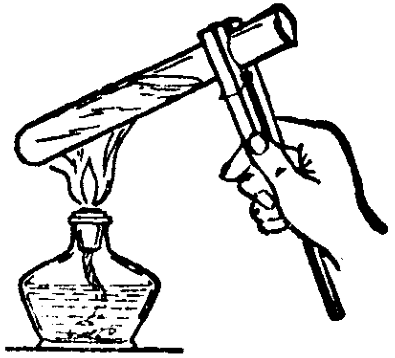
\includegraphics[width=4cm]{../pic/czhx1-xssy-25}
            \caption{\begin{minipage}[t]{4cm}
                用试管夹夹住\\
                试管进行加热
            \end{minipage}}\label{fig:xssy-25}
        \end{minipage}
        \qquad
        \begin{minipage}[b]{3cm}
            \centering
            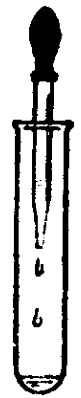
\includegraphics[width=1cm]{../pic/czhx1-xssy-26}
            \caption{\begin{minipage}[t]{2cm}
                用滴管滴\\
                加液体
            \end{minipage}}\label{fig:xssy-26}
        \end{minipage}
        \qquad
        \begin{minipage}[b]{5cm}
            \centering
            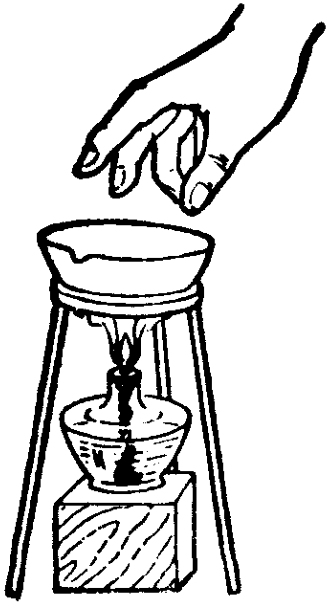
\includegraphics[width=4cm]{../pic/czhx1-xssy-27}
            \caption{\begin{minipage}[t]{4cm}
                移走正在加热\\
                的蒸发皿
            \end{minipage}}\label{fig:xssy-27}
        \end{minipage}
    \end{figure}
\end{wentihetaolun}


\section{土壤酸碱性的测定 几种化肥的性质}\label{sec:xssy-sy9}

\begin{shiyanmudi}
    1. 学会用 pH 试纸测定土壤的酸碱度的简单方法; 2. 认识几种常见化肥的性质。
\end{shiyanmudi}


\begin{shiyanyongpin}
    烧杯、pH 试纸、玻璃棒、试管、漏斗、滤纸、铁架台(带铁圈)、酒精灯、坩埚钳。

    碳酸氢铵、硫酸铵、硝酸铵、尿素、过磷酸钙、石灰水、熟石灰、木炭、土样、蒸馏水。
\end{shiyanyongpin}


\begin{shiyanbuzhou}
    1. 测定土壤的酸碱度

    取 10 克土样放在烧杯里, 加 10—15 毫升蒸馏水,充分搅拌后,静置使之沉淀,待悬浊液澄清后,
    用 pH 试纸一端浸入溶液里,立即取出,把试纸颜色跟比色卡对比,就可测出土壤的 pH 值。

    2. 几种常见化肥的性质

    (1) 把碳酸氢铵、硫酸铵、硝酸铵、尿素、过磷酸钙等五种化肥各取少量(约 $0.2$ 克),分别放入五个试管里,观察它们的颜色和状态。

    (2) 闻闻这五种化肥的气味,哪一个试管里有氨的气味,为什么?

    (3) 在 5 个试管里,各加入 10 毫升水,轻轻振荡,观察每种化肥是否容易溶于水。

    (4) 把过磷酸钙和水的混和物过滤,得到过磷酸钙的饱和溶液。向澄清的石灰水里加入过磷酸钙的饱和溶液,
    有什么现象发生?稍放置一会儿,是不是有沉淀产生?如果有沉淀产生,是什么?

    (5) 取上述五种化肥各少许放在纸上,分别跟少量熟石灰混和并研磨,哪种化肥产生氨的气味?

    (6) 取上述五种化肥各少许,分别在红热的木炭上灼烧,观察各有什么现象发生。
\end{shiyanbuzhou}


\begin{wentihetaolun}
    根据实验说明可以用什么方法检验铵盐。
\end{wentihetaolun}


\section{酸、碱、盐、氧化物的实验习题}\label{sec:xssy-sy10}

\begin{shiyanmudi}
    1. 巩固酸、碱、盐、氧化物四类物质彼此之间发生反应的知识; 2. 培养学生观察、思维、独立操作等能力和探讨问题的科学方法。
\end{shiyanmudi}


\begin{shiyanxiti}
    1. 怎样用氢氧化钙制取氯化钙。

    2. 怎样用三种方法制取硫酸镁。

    3. 怎样用氧化铜制取氢氧化铜? 怎样用氧化铜制取铜(不用氢气还原的方法)?

    4. 怎样鉴别硫酸镁溶液和氯化镁溶液?

    5. 用实验证明氧化钙能够跟水化合,而氧化铜不能跟水化合。

    6. 用实验证明铁、铜、银这三种金属的活动性顺序。

    7. 怎样鉴别水、盐酸、氢氧化钠溶液和氯化钠溶液。
\end{shiyanxiti}




\setcounter{section}{0}
\ctexset {
    section={
        name={选做实验,},
        number=\chinese{section},
    },
}
\section{测定硝酸钾在水里的溶解度并绘制它的溶解度曲线图\footnotemark}\label{sec:xssy-xzsy1}
\footnotetext{本实验编入了两种方法——溶质质量法和结晶析出法,教师可根据实际情况任选一种。
    选用溶质质量法时,可让每个实验小组分别测定一个温度下的溶解度,然后综合全班各组测出的数据,绘出溶解度曲线图。
    选用结晶析出法时,可让每个实验小组测两个温度下的溶解度。
}

\begin{shiyanmudi}
    1. 学会测定固体物质的溶解度,加深对溶解度概念的理解; 2. 学会溶解度曲线图的绘制方法; 3. 学会使用温度计和水浴加热的操作技能。
\end{shiyanmudi}


\begin{shiyanyongpin}
    托盘天平、烧杯(250 毫升)、试管、玻璃棒、温度计、酒精灯、量筒(10 毫升)、铁架台(带铁圈和铁夹)、蒸发皿、石棉网、干燥器、坩埚钳。

    硝酸钾、蒸馏水。
\end{shiyanyongpin}


\subsection{溶质质量法}


\begin{shiyanbuzhou}
    \begin{wrapfigure}[16]{r}{5cm}
        \centering
        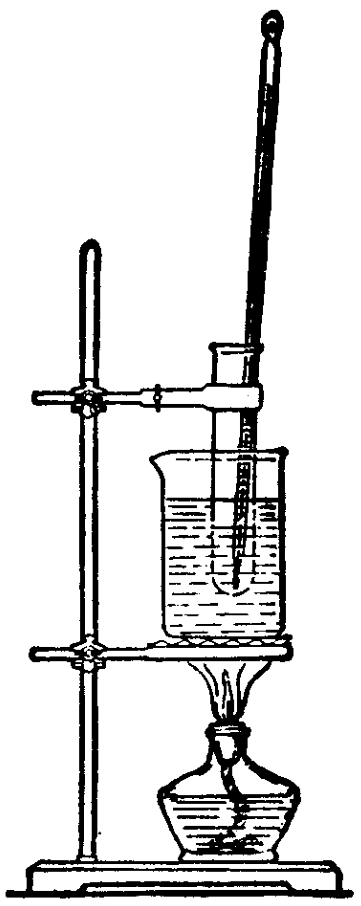
\includegraphics[width=3.5cm]{../pic/czhx1-xssy-28}
        \caption{测定溶解度}\label{fig:xssy-28}
    \end{wrapfigure}

    1. 用天平称量一个干燥的蒸发皿的质量,并将称量的数值记入下面的表里。

    2. 用量筒量取 10 毫升蒸馏水,倒入试管里。然后把一支温度计放在试管里(如图 \ref{fig:xssy-28} 所示 )。
    在烧杯里倒入约 150 毫升水,将试管(连水带温度计)放入烧杯里,进行水浴%
    \footnote{当被加热物质要求受热均匀时,而温度不能超过 100 ℃时,可利用水浴。}加热。
    利用酒精灯控制水温,使试管里温度保持相对稳定。\footnote{如果欲测温度是 20 ℃, 那么在 18 ~ 22 ℃ 时保持稳定也可以。}

    保持恒温后,逐渐向试管里加入少量硝酸钾的晶体,用玻璃棒搅拌,直到在五分钟内不再溶解为止。

    3. 取下试管,把里面的硝酸钾溶液倾倒在已称量过的蒸发皿里(注意不要把未溶解的硝酸钾晶体倒入)。
    然后称量,把数值记入下表里。

    4. 把蒸发皿放到酒精灯上加热,边加热边搅拌。待析出晶体较多时,改用微火加热,直到水分完全蒸发掉为止。
    待稍冷后,把蒸发皿放入干燥器中冷却,冷却后,称量,直到两次称量的质量结果相差不超过 $0.1$ 克。把数据记入下表中。

    5. 利用所测数据,根据下式计算出硝酸钾在指定的一个温度下的溶解度 $S$。

    \begin{tblr}{
        hlines, vlines,
        columns={c,m, 5em},
        column{1}={3em},
    }
        {温度\\[-.3em]℃}
            & {蒸发皿\\[-.5em]的质量\\[-.5em]$a$(克)}
            & {(蒸发皿\\[-.5em] $+$ 溶液)\\[-.5em]的质量\\[-.5em] $b$(克)}
            & {(蒸发皿\\[-.5em] $+$ 晶体)\\[-.5em]的质量\\[-.5em] $c$(克)}
            & {水的质量\\[-.5em] $b - c$(克)}
            & {晶体的质量\\[-.5em] $c - a$(克)}
            & {溶解度\\[-.5em] $S$(克)} \\
        \\
        \\
        \\
        \\
        \\
    \end{tblr}

    \jiange
    $$ \text{溶解度(克)} \; S = \dfrac{100(c - a)}{b - c} $$

    把本组和其它各组在不同温度下测定的数据分别填入上表里。
    欲测温度可分别选择为 10 ℃、20 ℃、30 ℃、40 ℃、50 ℃等。

    6. 根据所得到的数据,以温度为横坐标、溶解度为纵坐标,绘制溶解度曲线图。
\end{shiyanbuzhou}


\begin{wentihetaolun}
    1. 用水浴加热时,为什么一定要把试管内的液体全部浸没在水浴里?

    2. 测定硝酸钾的溶解度时,试管里除温度应保持恒定外,还应留有一些未溶解的硝酸钾,为什么?

    3. 为什么倾倒出来的饱和溶液里不能混有固体?

    4. 把你测得的溶解度跟课本中的溶解度数据进行比较,并作简单的分析。通过本实验,你有什么经验教训和体会?
\end{wentihetaolun}


\subsection{结晶析出法}

\begin{shiyanbuzhou}
    1. 在托盘天平上分别称量硝酸钾 2.5 克、3.5 克、5.0 克、7.0 克、9.0 克,
    然后依次放入已经编好号的干燥的试管里。注意不要把硝酸钾粘在试管壁上。

    2. 用量筒量取 10 毫升蒸馏水。在五个试管里分别加入 10 毫升蒸馏水。

    3. 在每个试管里插入一根玻璃棒,然后依次把每个试管放在水浴里进行加热,
    边加热边搅拌,使硝酸钾固体全部溶解。在加热过程中,要用温度计测水温。
    注意不要使温度上升过高,以致下一步结晶析出需要的时间太长\footnote{
        可以进行粗略计算。例如,20 ℃ 时硝钾溶解度为 31.6 克,那么 20 ℃ 时在 10 毫升水里最多能溶解 3.16 克硝酸钾。
        2 号试管中有 3.5 克硝酸钾,大约在略高于 20 ℃ 时能全部溶解,因此加热温度不要高于 30 ℃,以此类推。
    }。

    4. 当硝酸钾全部溶解后,可把试管拿出水面,插入一根干净的温度计,
    一边用玻璃棒轻轻地摩擦管壁,一边观察温度计的读数。
    这时一定要耐心和细心,当有晶体析出时,立即读取温度,并作记录。

    5. 把试管再放入水浴里加热,使硝酸钾溶解。然后重复上面的操作,再测定晶体析出时的温度。
    对比两次的读数,如果差别较大,再重复测定一次。

    6. 根据所测数据,计算硝酸钾的溶解度。

    \begin{tblr}{
        hlines, vlines,
        columns={c},
        column{4-6}={3em},
    }
        \SetCell[r=2]{m} 编号
            & {\SetCell[r=2]{m} 硝酸钾的质量\\(克)}
            & \SetCell[r=2]{m} {水的体积\\(毫升)}
            & \SetCell[c=3]{c} 结晶析出的温度(℃) & &
            & \SetCell[r=2]{m} {溶解度\\(克)} \\
        & & & 1 & 2 & 平均值 & \\
        1 & 2.5 & 10 & & & & \\
        2 & 3.5 & 10 & & & & \\
        3 & 5.0 & 10 & & & & \\
        4 & 7.0 & 10 & & & & \\
        5 & 9.0 & 10 & & & & \\
    \end{tblr}


    \jiange
    7. 根据所得到的数据,以温度为横坐标、溶解度为纵坐标,绘制溶解度曲线图。
\end{shiyanbuzhou}


\begin{wentihetaolun}
    把你测得的溶解度跟课本中的溶解度数据进行比较,并作简单的分析。通过本实验,你有什么经验教训和体会?
\end{wentihetaolun}



\section{制取硫酸铜晶体}\label{sec:xssy-xzsy2}

\begin{shiyanmudi}
    1. 学习通过化学反应制取硫酸铜晶体的方法; 2. 巩固对酸的性质的认识。
\end{shiyanmudi}


\begin{shiyanyongpin}
    铁架台(带铁圈)、蒸发皿、坩埚钳、玻璃棒、烧杯、量筒、酒精灯、漏斗、滤纸、剪刀、药匙。

    氧化铜、稀硫酸($1:4$)。
\end{shiyanyongpin}


\begin{shiyanbuzhou}
    1. 用量筒量取 15 毫升稀硫酸倒入一个蒸发皿里,把蒸发皿放在铁架台的铁圈上,
    用酒精灯加热到将近沸腾(但不要使稀硫酸沸腾)。然后注意保持这个温度,
    一边用玻璃棒进行搅拌,一边慢慢地撒入氧化铜粉末,直到氧化铜不再溶解为止。
    记录观察到的现象,并写出反应的化学方程式。

    2. 装置好漏斗,趁热\footnote{硫酸铜在水中的溶解度(克)\\[.5em]
        \begin{tblr}{hlines, vlines,columns={c,colsep=1em}}
                       & 0 ℃ & 20 ℃ & 40 ℃ & 60 ℃ & 80 ℃ \\
            \ce{CuSO4} & 14.3 & 20.7 & 28.5 & 40  & 55 \\
        \end{tblr}
    }
    过滤(过滤时,不溶性物质可以留在蒸发皿里,不必转移到滤纸上)。将滤液收集在烧杯里。

    3. 使滤液逐渐冷却,仔细观察晶体生成时所发生的现象,并记录晶体的颜色和形状。
    如果滤液放置一段时间后,没有晶体生成,可以把滤液倒入洗净的蒸发皿里蒸发几分钟,
    再放置冷却,就会有晶体生成。
\end{shiyanbuzhou}


\begin{wentihetaolun}
    1. 为什么要趁热过滤? 等液体冷后再过滤会出现什么现象?

    2. 如果过滤速度太慢会发生什么情况? 在实验时应怎样做好过滤前的准备工作?
\end{wentihetaolun}



\endgroup

